\documentclass[preprint,3p]{elsarticle}
%\documentclass[preprint]{aastex}
\usepackage{aas_macros}
\usepackage{amsmath,amssymb}
\usepackage{mathrsfs}
\usepackage{graphicx}
\usepackage{bm}
\usepackage{hyperref}
\DeclareMathOperator\erf{erf}
\newcommand{\mli}[1]{\mathit{#1}}
%\usepackage{epstopdf}


\begin{document}

%\begin{frontmatter}
%
%\title{Toy Model}
%\author{A.~G. Kim\corref{cor1}}
%\ead{agkim@lbl.gov}
%\address{Physics Division, Lawrence Berkeley National Laboratory, 1 Cyclotron Road, Berkeley CA, USA 94720}
%
%\begin{abstract}
%\end{abstract}
%\begin{keyword}
%\end{keyword}
%\end{frontmatter}

\section{Likelihood and Posterior}
\label{likelihood:sec}

The ambition is to construct a model to determine the likelihood of DES-like
supernova data. 
The conceptual structure of the model is shown in Figure~\ref{pgm:fig}. 
\begin{figure}[htbp] %  figure placement: here, top, bottom, or page
   \centering
   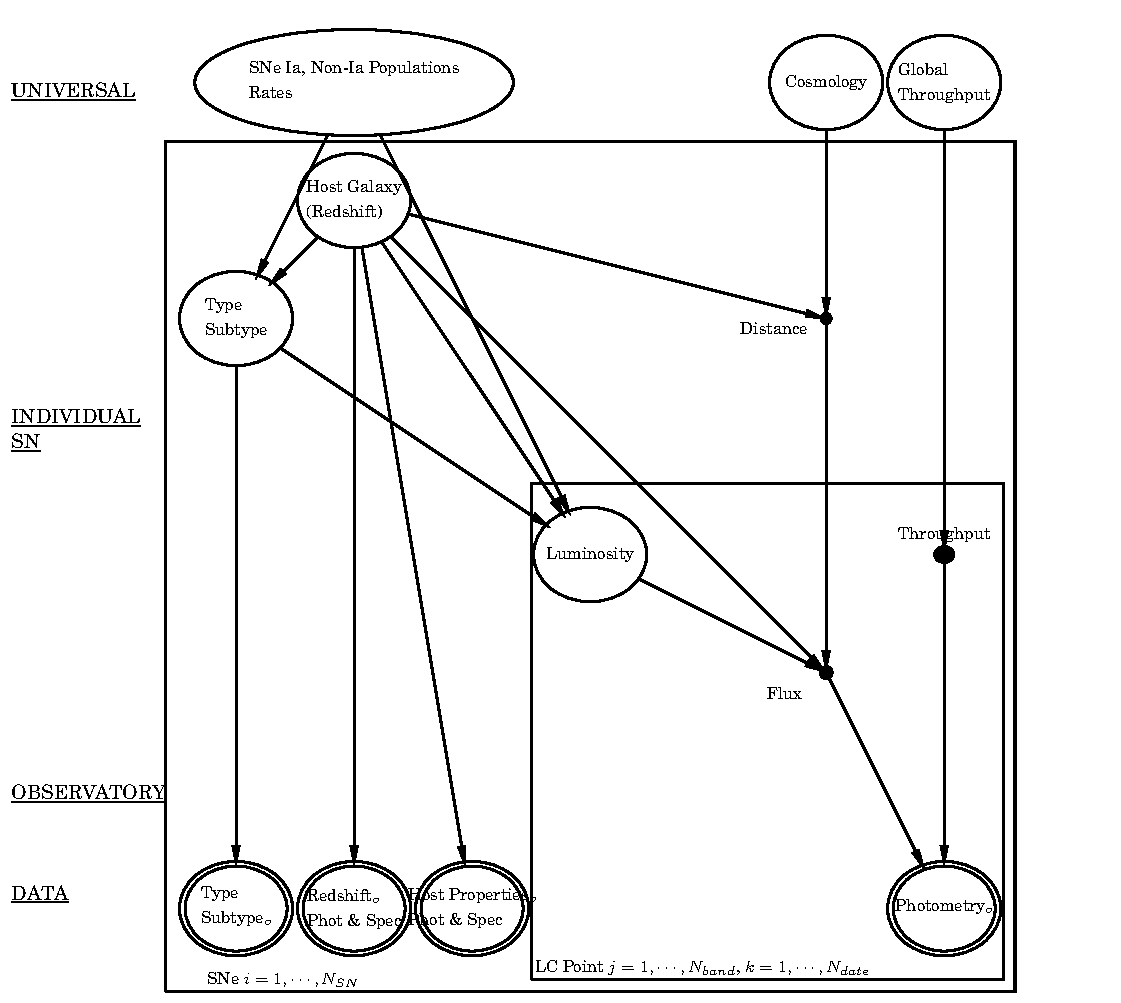
\includegraphics[width=6.5in]{../results//hdpgm.pdf} 
   \caption{Probabilistic Graphical Model for the SN~Ia analysis.  
   \label{pgm:fig}}
\end{figure}

The model has three types of observables $O$ that
may be observed for each supernova:
\begin{itemize}
\item $c$: Counts of the photometric measurements (light curves).
\item $s$: Counts of the spectroscopic measurements.
\item $z$: Redshift.
\item $T$: Transient type.
\end{itemize}
The measurements made of the observables are labeled  with a subscript ``o''.

There are top-level  sets of parameters $M$ that correspond to photometric calibration, cosmology,
host-galaxy properties, and transient properties.
There are two sets of intermediary parameters $M_I$ that correspond to luminosity $L$ and type $\tau$.

Not all transients that occur in nature will be detected or pass our sample cuts, and the parameter pdf's
depend on the sample under consideration: the $S$ subscript specifies a pdf for the analysis sample,
whereas the $p$'s with no subscript specifies the pdf of the underlying sample.
The likelihood for observations $O_o$ is expressed as
\begin{align*}
\mathcal{L}_S(O_o | M, M_I) & = \frac{\epsilon(O_o, M, M_I) p(O_o|M, M_I)}{\int  \epsilon(O, M, M_I) p(O|M, M_I)dO},
\end{align*}
$p(O|M, M_I)$ is the pdf of the underlying sample, and $\epsilon(O, M, M_I) $
is the probability those observables will be included in the analysis sample.
As the observable uncertainties
are expected to be independent between different transients we can decompose the likelihood into terms
for each.
\begin{align*}
\mathcal{L}_S(O_o | M, M_I) & = \frac{\prod_{\alpha \in transients} \epsilon(O_o^\alpha, M, M_I) p(O_o^\alpha|M, M_I)}{\int \prod_{\alpha \in transients}  \epsilon(O^\alpha, M, M_I) p(O^\alpha|M, M_I)dO^\alpha}.
\end{align*}
Note that we work with counts: for fluxes this splitting would not be possible due to correlated calibration uncertainties.

We now consider the terms of the likelihood contributed by each transient and omit the $\alpha$ superscript. 
The dependencies of the parameters are charted through the PGM to give for transients with a type measurement
\begin{align*}
p(O| M, M_I) & = P(T | \tau) p(z | M) p(c | L, M) p(s|L, M)
\end{align*}
and for transients without a type measurement (not relevant for the SN~Ia-only analysis but included for completeness)
\begin{align*}
p(O| M, M_I) & = p(z | M) p(c | L, M),
\end{align*}
where the observations are taken to have measurement uncertainties that are independent.  

The efficiency $\epsilon(O, M, M_I) $ depends on the properties of the experiment and the sample selection criteria:
the transient is discovered, satisfies sample selection, is selected for spectroscopic typing, the typing
is successful, and that the type is SN~Ia:
\begin{align*}
\epsilon(O, M, M_I)  & = P(SNIa, typed, spec, sample, discovered |O, M, L, \tau)\\
& = P(SNIa|  typed, \tau)P(typed | spec, s, M, M_I)P(spec | discovered, c) \\
& \times P(sample| discovered, c)P(discovered |c).
\end{align*}
Transient discovery and sample selection are purely based on observed photometry $c$.
The decision for spectroscopic follow-up is also based on observed photometry,  though perhaps external redshift estimates
of the possible host galaxy may come into play.  The success of the typing measurement should primarily depend
on the signal $s$, but may also depend on the type and host properties.  For the pure SN~Ia sample under initial consideration
the first term is 1.

A frequentist analysis can proceed with this likelihood.
Alternatively, the Bayesian posterior is specified by parameter priors as follows:
\begin{align*}
p(M, M_i | O_o) & \propto \mathcal{L}_S(O_o| M, M_I) p(M_I|M) p(M)\\
 & \propto \mathcal{L}_S(O_o| M, M_I) p(L| \tau, M) p(\tau|M) p(M).
\end{align*}
Once all the $p$'s and $P$'s are specified we are ready to analyze!

\section{Probabilities}
Section~\ref{likelihood:sec} introduces the probabilities and probability distribution functions that describe the likelihood
and posterior for the model shown in Figure~\ref{pgm:fig}.
In this Section we present one possible model by specifying those probabilities; the assembly of other models should
resemble this example.

\subsection{$p(M)$: Priors on the Top-Level Parameters}
\begin{itemize}
\item
Flat $w$CDM cosmological parameters are drawn from top-hat distributions
\begin{align}
\Omega_M & \sim  {\mathcal{U}}(0,1)\\
w_0 & \sim \mathcal{U}(-1.5, -0.1).
\end{align}

\item
Photometric zeropoints for each band are given by
\begin{equation}
Z \sim \mathcal{N}\left(0,\left(\frac{\ln{10}}{2.5}\right)^2 C_{cal}\right),
\end{equation}
where $C_{cal}$ is the covariance of the calibration zeropoints that Chris Lidman is calculating.

\item
There are a number of parameters that describe the supernova populations.

The luminosity of SNe~Ia as a function of time and wavelength is described by the SALT2 model and
the linear relation of its parameters with absolute magnitude.
There are parameters for the global supernova parameters.  For SNe~Ia
\begin{align}
M_{SNIa} & \sim \mathcal{U}(-20, -18) \\
\arctan{\alpha_{SNIa}} & \sim \mathcal{U}(-0.2, 0.3) \\
\arctan{\beta_{SNIa}} & \sim \mathcal{U}(-1.4, 1.4),
\end{align}
where $M_{SNIa} = -2.5\log_{10}({L_{SNIa}})$
and for ``hyperparameters'' that describe the distributions of the per-supernova parameters
\begin{align}
\log_{10}{R^{x_0}_{SNIa}} & \sim \mathcal{U}({-2}, {-0.5})\\
\log_{10}{R^{x_1}_{SNIa}} & \sim \mathcal{U}({-0.5}, {0.5})\\
\log_{10}{R^{c}_{SNIa}} & \sim \mathcal{U}({-1.5}, {-0.5})\\
x_{1,SNIa}^\star& \sim \text{Cauchy}(0,1)\\
c^\star_{SNIa} & \sim \text{Cauchy}(0,0.3).
\end{align}

The following aspects of the model are irrelevant for the cosmology analysis of the pure SN~Ia sample
but are presented for completeness.

We take the rates relative to the SN~Ia rate
\begin{equation}
r_{SNIa} = 1.
\end{equation}
If we were interested in the absolute rates this term could be replaced with your favorite parameterized
SN rate model.
The relative non-Ia rate would be a stochastic parameter, with a prior
\begin{equation}
r_{SNII} \sim \mathcal{U}(0.25, 4).
\end{equation}
In a better model this relative rate would be redshift-dependent.

When considering the photometric sample the model needs to consider non-Ia populations.
We defer discussion on what model is used for non-Ia's for the moment.

\item 
In the photometric-sample analysis a prior must be specified for the redshift.  The redshift is drawn from a flat distribution
\begin{equation}
z\sim \mathcal{U}(0,\infty).
\end{equation}
\end{itemize}

\subsection{$p(M_I|M)$: Probabilities of the Intermediary Parameters.}
\begin{itemize}
\item Type probabilities are relevant in the photometric analysis.
The probability an object is SN~Ia is
\begin{align}
p_{SNIa} &= \frac{r_{SNIa}}{r_{SNIa}+r_{SNII}} \nonumber \\
p_{SNII}&=1-p_{SNIa}.
\label{prob:eqn}
\end{align}

The type of the object $\tau$ is drawn from the Bernoulli distribution 
\begin{equation}
\tau | p_{SNIa} \sim \mathcal{B}(1-p_{SNIa}),
\end{equation}
with the convention that $T=0$ corresponds to SN~Ia.


Now we have the parameters that specify the sub-type.
\begin{align}
t_0 & \sim \mathcal{U}\\
x_{0, SNIa} & \sim \mathcal{N}(0,R^{x_0}_{SNX})\\
x_{1,SNIa} & \sim \mathcal{N}(x_{1,SNIa}^\star,R^{x_1}_{SNIa})\\
c_{SNIa} & \sim \text{SkewNormal}(c^\star_{SNIa},R^{c}_{SNIa} )
\end{align}

\end{itemize}

\subsection{$p(O| M, M_I)$: Probability of All Possible Observables}
\begin{itemize}
\item The spectroscopic typing is assumed to be perfect
\begin{equation}
T | \tau \sim \delta (T-\tau).
\end{equation}

\item The spectroscopic redshift of a spectroscopically typed transient assumed to be perfect
\begin{equation}
z | z_{host} ~ \delta (z-z_{host}).
\end{equation}

When the transient is not spectroscopically typed, there is ambiguity in the correct assignment of the host galaxy.
Then the measured redshift is a sum of delta functions
\begin{equation}
p(z_o|z) = \sum_i p_i \delta(z-z_i),
\end{equation}
where galaxy $i$ at
redshift $z_i$ has probability $p_i$ of being
the host.  

\item  The luminosity distance comes from the physics-theory function
\begin{equation}
d_L = d_L(z; \Omega_M, w0),
\end{equation}
the flux for an observation at date $t$ is
\begin{equation}
f = 10^{-0.25 \left(M - \alpha x_1 + \beta c \right)}\frac{1}{4\pi d_L^2} F_{SALT2}((t-t_0)/(1+z); x_0,  x_1, c, \lambda/(1+z)),
\end{equation}
and expected counts is
\begin{equation}
c_\star = 10^{Z/2.5}f.
\end{equation}
The distribution of counts for all transients is 
\begin{equation}
c | c_\star, \sigma_c \sim \mathcal{N}(c_\star, \sigma_c),
\end{equation}
where $\sigma_c$ is the measurement noise.

\end{itemize}

\subsection{$\epsilon(O, M, M_I)$: Sample Inclusion Efficiency}
The probability that a transient becomes a part of the analysis sample is given by $\epsilon(O, M, M_I)$ and is dependent
on the properties of the experiment and choices made by the experimenter.

\begin{itemize}
\item The probability the transient is discovered is given by
$P(discovered |c)$.  To first order, the discovery probability within a single image depends on the transient signal-to-noise $\epsilon(STON)$.  For
an image with noise $N$ and observable counts the efficiency is then $\epsilon(c/N)$.  The probability of discovery in at least one image is
thus
\begin{equation}
P(discovered |c)= 1-\prod_{\beta \in images} \left(1-\epsilon(c_\beta/N_\beta)\right).
 \end{equation}
\item Typically not all discoveries, but only transients that satisfy sample selection criteria are included in the cosmology
analysis.  For example, the object must have pass minimum signal-to-noise requirements in several bands and phases.
The probability that a discovered transient is included in the sample is $P(sample| discovered, c)$.
We could do a simulation to determine this function.
\item Alternatively we could replace  $P(sample| discovered, c)P(discovered |c)$ with
\begin{equation}
P(discovered | sample, c)P(sample |c).
\end{equation}
If the sample selection criteria are selected such that $P(discovered | sample, c)=1$ (validated through simulation) then
$P(sample |c)$ becomes the sum of  configurations of products of step functions and Gaussians.  This has significant
computational benefits.
\item The probability of obtaining a spectroscopic observation of a transient is given as $P(spec | discovered, c)$.  Each follow-up telescope
has its own criteria: OzDES is magnitude limited, VLT prefers transients on faint hosts, others may try to get a random sample uniform in
redshift.
\item The probability that the spectroscopic observation yields a type is $P(typed | spec, s, M, M_I)$.  This is a function we have to
figure out!
\item This term appears for the typed SN~Ia sample, where it is trivial $P(SNIa|  typed, \tau)=1$.
\end{itemize}

%\subsection{Case Typed}
%For Case Typed the likelihood is
%\begin{align}
%\mathcal{L}(T_o,z_o,c_o | S_c, S_T, z, X) & =  \int dL \sum_i p(T_o,z_o,c_o | T_i, L, S_c, S_T, z, X) p(L |  T_i,  S_c, S_T, z, X) P(T_i|S_c, S_T, z, X).
%\end{align}
%We assume that the observations give a perfect measurement of type and redshift,
%so that
%\begin{align}
%p(T_o|T) & =\delta(T_o-T)\\
%p(z_o|z) & =\delta(z_o-z);
%\end{align}
%$T$ and $z$ are no longer probabilistic but are fixed.
%Then
%\begin{align}
%\mathcal{L}(T_o,z_o,c_o | S_c, S_T, z, X) & =  \int dL\, p(c_o | T=T_o, L, S_c, S_T, z=z_o, X) p(L| T=T_o, S_c, S_T, z=z_o, X)  P(T_o|S_c, S_T, z=z_o, X) \\
%&= \int dL\, \frac{ p(c_o, S_c, S_T | T=T_o, L, z=z_o, X) }{P(S_c, S_T, | T=T_o, L,  z=z_o, X) }
%\frac{p(L, S_c, S_T | T=T_o, z=z_o, X)}{P(S_c, S_T| T=T_o,  z=z_o, X)}
%\frac{p(T_o, S_c, S_T | z=z_o, X)}{P(S_c, S_T| z=z_o, X)} \\
%&= \frac{\int dL\, p(L|T_o, z=z_o, X) P(T_o|z=z_o, X) p(c_o, S_c, S_T | T=T_o, L, z=z_o, X)}{P(S_c, S_T| z=z_o, X)}.%\\
%%&= \frac{\int dL\, p(L|T_o, z=z_o, X) P(T_o|z=z_o, X) p(c_o | T=T_o, L, z=z_o, X)}{P(S_c, S_T| z=z_o, X)}.
%\end{align}
%
%The photometric and spectroscopic sample selections can be treated as efficiencies $\epsilon_c$, $\epsilon_T$ as
%\begin{align}
%p(c_o, S_c, S_T | T=T_o, L, z=z_o, X) & = \int ds\, p(c_o, s, S_c, S_T | T=T_o, L, z=z_o, X) \\
% & =p(c_o, S_c | T=T_o, L, z=z_o, X)  \int ds\,  p(s, S_T | T=T_o, L, z=z_o, X) \\
% & = \epsilon_c(c_o) p(c_o| T=T_o, L, z=z_o, X)  \int ds\, \epsilon_T(c_o, s)  p(s | T=T_o, L, z=z_o, X) \\
% & \approx \epsilon_c(c_o)   \epsilon_T(c_o, s_\star) p(c_o| T=T_o, L, z=z_o, X).
%\end{align}
%where the supernova signal in the spectrum $s$ is not extracted and we make the approximation $ p(s | T=T_o, L, z=z_o, X)  = \delta(s-s_\star)$
%and $s_\star(t_T; T=T_o, L, z=z_o, X)$ is the expected signal.
%
%
%The  normalization term sums/integrates over all possible observed types/counts 
%\begin{align}
%P(S_c, S_T| z=z_o, X) & =\sum_i \int dc_o \mathcal{L}(T_i,z_o,c_o | S_c, S_T, z, X) \\
%% & =\sum_i \int_{-\infty}^{\infty} dc_o \mathcal{L}(T_i,z_o,c_o | S_c, S_T, z, X) \\
%%& = \sum_i \int_{c_T}^{\infty} dc_o \mathcal{L}(T_i,z_o,c_o | S_c, S_T, z, X)\\
%& = \sum_i  P(T_i|z=z_o, X)\int dL\, p(L|T_i, z=z_o, X)  \left[\int dc_o\,  p(c_o,S_c, S_T | T=T_i, L, z=z_o, X)\right] \\
%& \approx  \sum_i   P(T_i|z=z_o, X)\int dL\, p(L|T_i, z=z_o, X)  \left[ \int dc_o\, \epsilon_c(c_o)  \epsilon_T(c_o, s_\star)  p(c_o| T=T_o, L, z=z_o, X)  \right] .
%\end{align}
%
%\subsection{Case Not Typed}
%
%
%For Case Not Typed the likelihood is
%\begin{align}
%\mathcal{L}(z_o,c_o | S_c, S_T, z, X) & =  \int ds \,\mathcal{L}(z_o,c_o, s | S_c, S_T, z, X) \\
%& =  \int ds \, \int dL \, \sum_i p(z_o,c_o, s | T_i, L, S_c, S_T, z, X) p(L |  T_i,  S_c, S_T, z, X) P(T_i|S_c, S_T, z, X).
%\end{align}
%
%For the redshift measurement, we take a set of potential host galaxies, where galaxy $j$
%are redshift $z_j$ has probability $p_j$ of being the host
%\begin{equation}
%p(z_o|S_c, S_T, z, X) = \sum_j   p_j\delta(z_j-z).
%\end{equation}
%Then
%\begin{align}
%\mathcal{L}(z_o,c_o | S_c, S_T, z, X) & =  \sum_j p_j \int ds \, \int dL \,\sum_{i} p(c_o | T_i, L, S_c, S_T, z=z_j, X) p(s | T_i, L, S_c, S_T, z=z_j, X) \\
%& \times p(L |  T_i,  S_c, S_T,  z=z_j, X) P(T_i|S_c, S_T, z=z_j, X) \\
%& \propto  \sum_j p_j \int ds \, \int dL \,\sum_{i} p(c_o, S_c, S_T | T_i, L, z=z_j, X) p(s, S_c, S_T | T_i, L, S_c, S_T, z=z_j, X) \\
%& \times p(L,, S_c, S_T |  T_i,  S_c, S_T,  z=z_j, X) P(T_i|S_c, S_T, z=z_j, X) \\
%&=  \frac{\sum_j p_j \int dL \, p(c_o, S_c, S_T | L, z=z_j, X) \sum_{i}  p(L|T_i, z=z_j, X) P(T_i|z=z_j, X)   }{P(S_c, S_T| z=z_j, X)}\\
%&=  \frac{\sum_j p_j \int dL \, p(c_o | L, z=z_j, X) \sum_{i}  p(L|T_i, z=z_j, X) P(T_i|z=z_j, X)   }{P(S_c, S_T| z=z_j, X)},
%\end{align}
%where we use the fact that the counts do not directly depend on type.
%
%The normalization term is
%\begin{align}
%P(S_c| z=z_o, X) & = \int dc_o \, \mathcal{L}(T_i,z_o,c_o | S_c, S_T, z, X)\\
%& =  \sum_j p_j  \sum_{i} P(T_i|z=z_j, X)  \int dL \, p(L|T_i, z=z_j, X) 
%\left[ \int dc_o \, p(c_o, S_c| T=T_i, L, z=z_j, X) \right].
%\end{align}

%\subsection{Sample Selection}
%Both the Typed and Not Typed cases have in their normalizations the term
%\begin{equation}
%\int dc_o \, p(c_o,S_c, S_T | T=T_i, L, z=z_o, X),
%\end{equation}
%which is the fraction of objects whose counts satisfy the sample selection criteria.
%
%
%In the case of a single count measurement per transient and neglecting the typing selection criteria,
%\begin{align}
% p(c_o, S_c, S_T | T=T_o, L, z=z_o, X) &=  p(c_o, c_o \ge  c_T | T=T_o, L, z=z_o, X) \\
% &= \begin{cases}
%   p(c_o | T=T_o, L, z=z_o, X) & \text{if } c_o \ge c_T \\
%   0 & \text{if }  c_o < c_T
% \end{cases}
%\end{align}
%so that the integral is
%\begin{equation}
%\int dc_o \, p(c_o,S_c, S_T | T=T_i, L, z=z_o, X) = \int_{c_T}^\infty dc_o\,  p(c_o | T=T_i, L, z=z_o, X).
%\end{equation}
%Our count measurements come from a Normal distribution, so that integral is simply related to the error function.
%
%For the more general case, suppose a transient has $N$ independent count measurements\footnote{The independence of count measurements  depends on the flux extraction method; regardless the
%noise of a single observation is expected to be dominated by its own photon noise making this
%supposition a good approximation.} and $k$ of those must be above threshold in order to be
%included in the sample.
%Consider arrays of length $N$ in which each element has a value of True or False: there are $2^N$ possible configurations for this array
%of which $\sum_{i=k}^N {N \choose i}$ have $k$ or more True's.  Let the set $\mathcal{G}$ represent the latter possible configurations.
%Then
%\begin{align}
%p(c_o, S_c| T=T_o, L, z=z_o, X) &= \sum_{g \in \mathcal{G}} \prod_{\alpha} p(c_{o, \alpha}, g | T=T_o, L, z=z_o, X)\\
% &=  \sum_{g \in \mathcal{G}}  \prod_{\alpha} \begin{cases}
%   p(c_{o,\alpha} | T=T_o, L, z=z_o, X) & \text{if } (c_{o,\alpha} \ge c_T) = g_\alpha\\
%   0 & \text{if }  (c_{o,\alpha} \ge c_T)  \ne g_\alpha
% \end{cases}
%\end{align}
%and the normalization integral is composed of the sum over all possible configurations of the integrated probability of the truncated distributions
%of the measured counts.  This simplifies to the the single-count case considered earlier in the case of $N=1$, $k=1$.
%If the count measurement uncertainties are independent, which may not be exactly but is approximately the case when we have high
%signal-to-noise references, the integral because a sum of products of normalized error functions.


\section{Implementation Notes}
Anticipating the use of available statistical packages, the likelihoods have been constructed
from standard distribution functions.  The truncated distributions from sample selection
are accounted by the normalization 
terms $P(S_c, S_T| z=z_o, X)$, $P(S_c| z=z_o, X)$.  Although they do not appear
in the PGM, they are treated as nodes who contribute 
$-\ln{P(S_c, S_T| z=z_o, X)}$ to the log-likelihood, where the negative sign reflects that this is a normalization
factor.


The following integral appears in the normalization
\begin{equation}
\int dL\, p(L|T_i, z=z_o, X)  \left[\int_{c_T}^{\infty} dc_o  p(c_o | T=T_i, L, z=z_o, X)\right].
\end{equation}
We actually work with $\ln{L_X}$ and $\sigma_X$.  Setting
\begin{equation}
n=\frac{\ln{L}-\ln{L_X}}{\sigma_X}
\end{equation}
the integral becomes
 \begin{equation}
\sigma_X \int dn\, p(n\sigma_X + \ln{L_X} |T_i, z=z_o, X)  \left[\int_{c_T}^{\infty} dc_o\,  p(c_o | T=T_i, L_Xe^{n\sigma_X}, z=z_o, X)\right].
\end{equation}
The two probability distributions are normal so that this reduces to
 \begin{equation}
\frac{1}{2\sqrt{2\pi}} \int dn\, e^{-0.5n^2} \left(1-erf\left(\frac{(c_T - c_\star)}{\sqrt{2}\sigma_c}\right)\right),
\end{equation}
where
\begin{equation}
c_\star = \frac{e^{\ln{L_X}+n\sigma_X}}{4\pi d_L^2}10^{Z/2.5}.
\end{equation}

\end{document}